
% ====================================
% chapter 2
% ====================================

\chapter{TeXでよく使うコマンド}

\section{セクション}

\verb|\section|をつけるとセクションわけができる.小分けにしたいときに便利.
\subsection{subsection}
さらに,\verb|\subsection|みたいに、さらなる小分けもできます.\verb|\subsubsection|みたいにsubをつけるほど細かくできます.

\subsection{サブセクションのテスト}

階層が深くなります.

\subsubsection{subsubsection}

めっちゃ階層が深くなります.
subをつけまくるとわかりにくくもなるのであまり階層を深くしすぎないように注意しましょう.

\section{図}

図は別フォルダにまとめておくと便利ですので,本テンプレートではFigというフォルダを作ってその中に図を入れています.

図は次のように出力します.
タイトル名やオプションなどは必要なように書き換えてください(詳しくはWebで!).
\begin{verbatim}
\begin{figure}[指定位置]
    \centering
    \includegraphics[オプション]{ファイル名}
    \caption{タイトル名} %タイトルをつける
    \label{ラベル} %ラベルをつけ図の参照を可能にする
\end{figure}
\end{verbatim}


修論のように大型の論文の場合は,Figフォルダの中で,更にフォルダを小分けしておくと便利です.
ここで,涅槃像を見にいった時に見つけた地蔵の画像を「Fig/ch2/地蔵.jpg」に入れてあるので,出力してみたいと思います(図\ref{fig_地蔵}).
画像が大きいのでオプション"scale"でサイズ調整してます.
ちなみに\verb|\ref{}|を使い{}内にラベル名を書くと番号を引用できます.

\begin{verbatim}
\begin{figure}[]
    \centering
    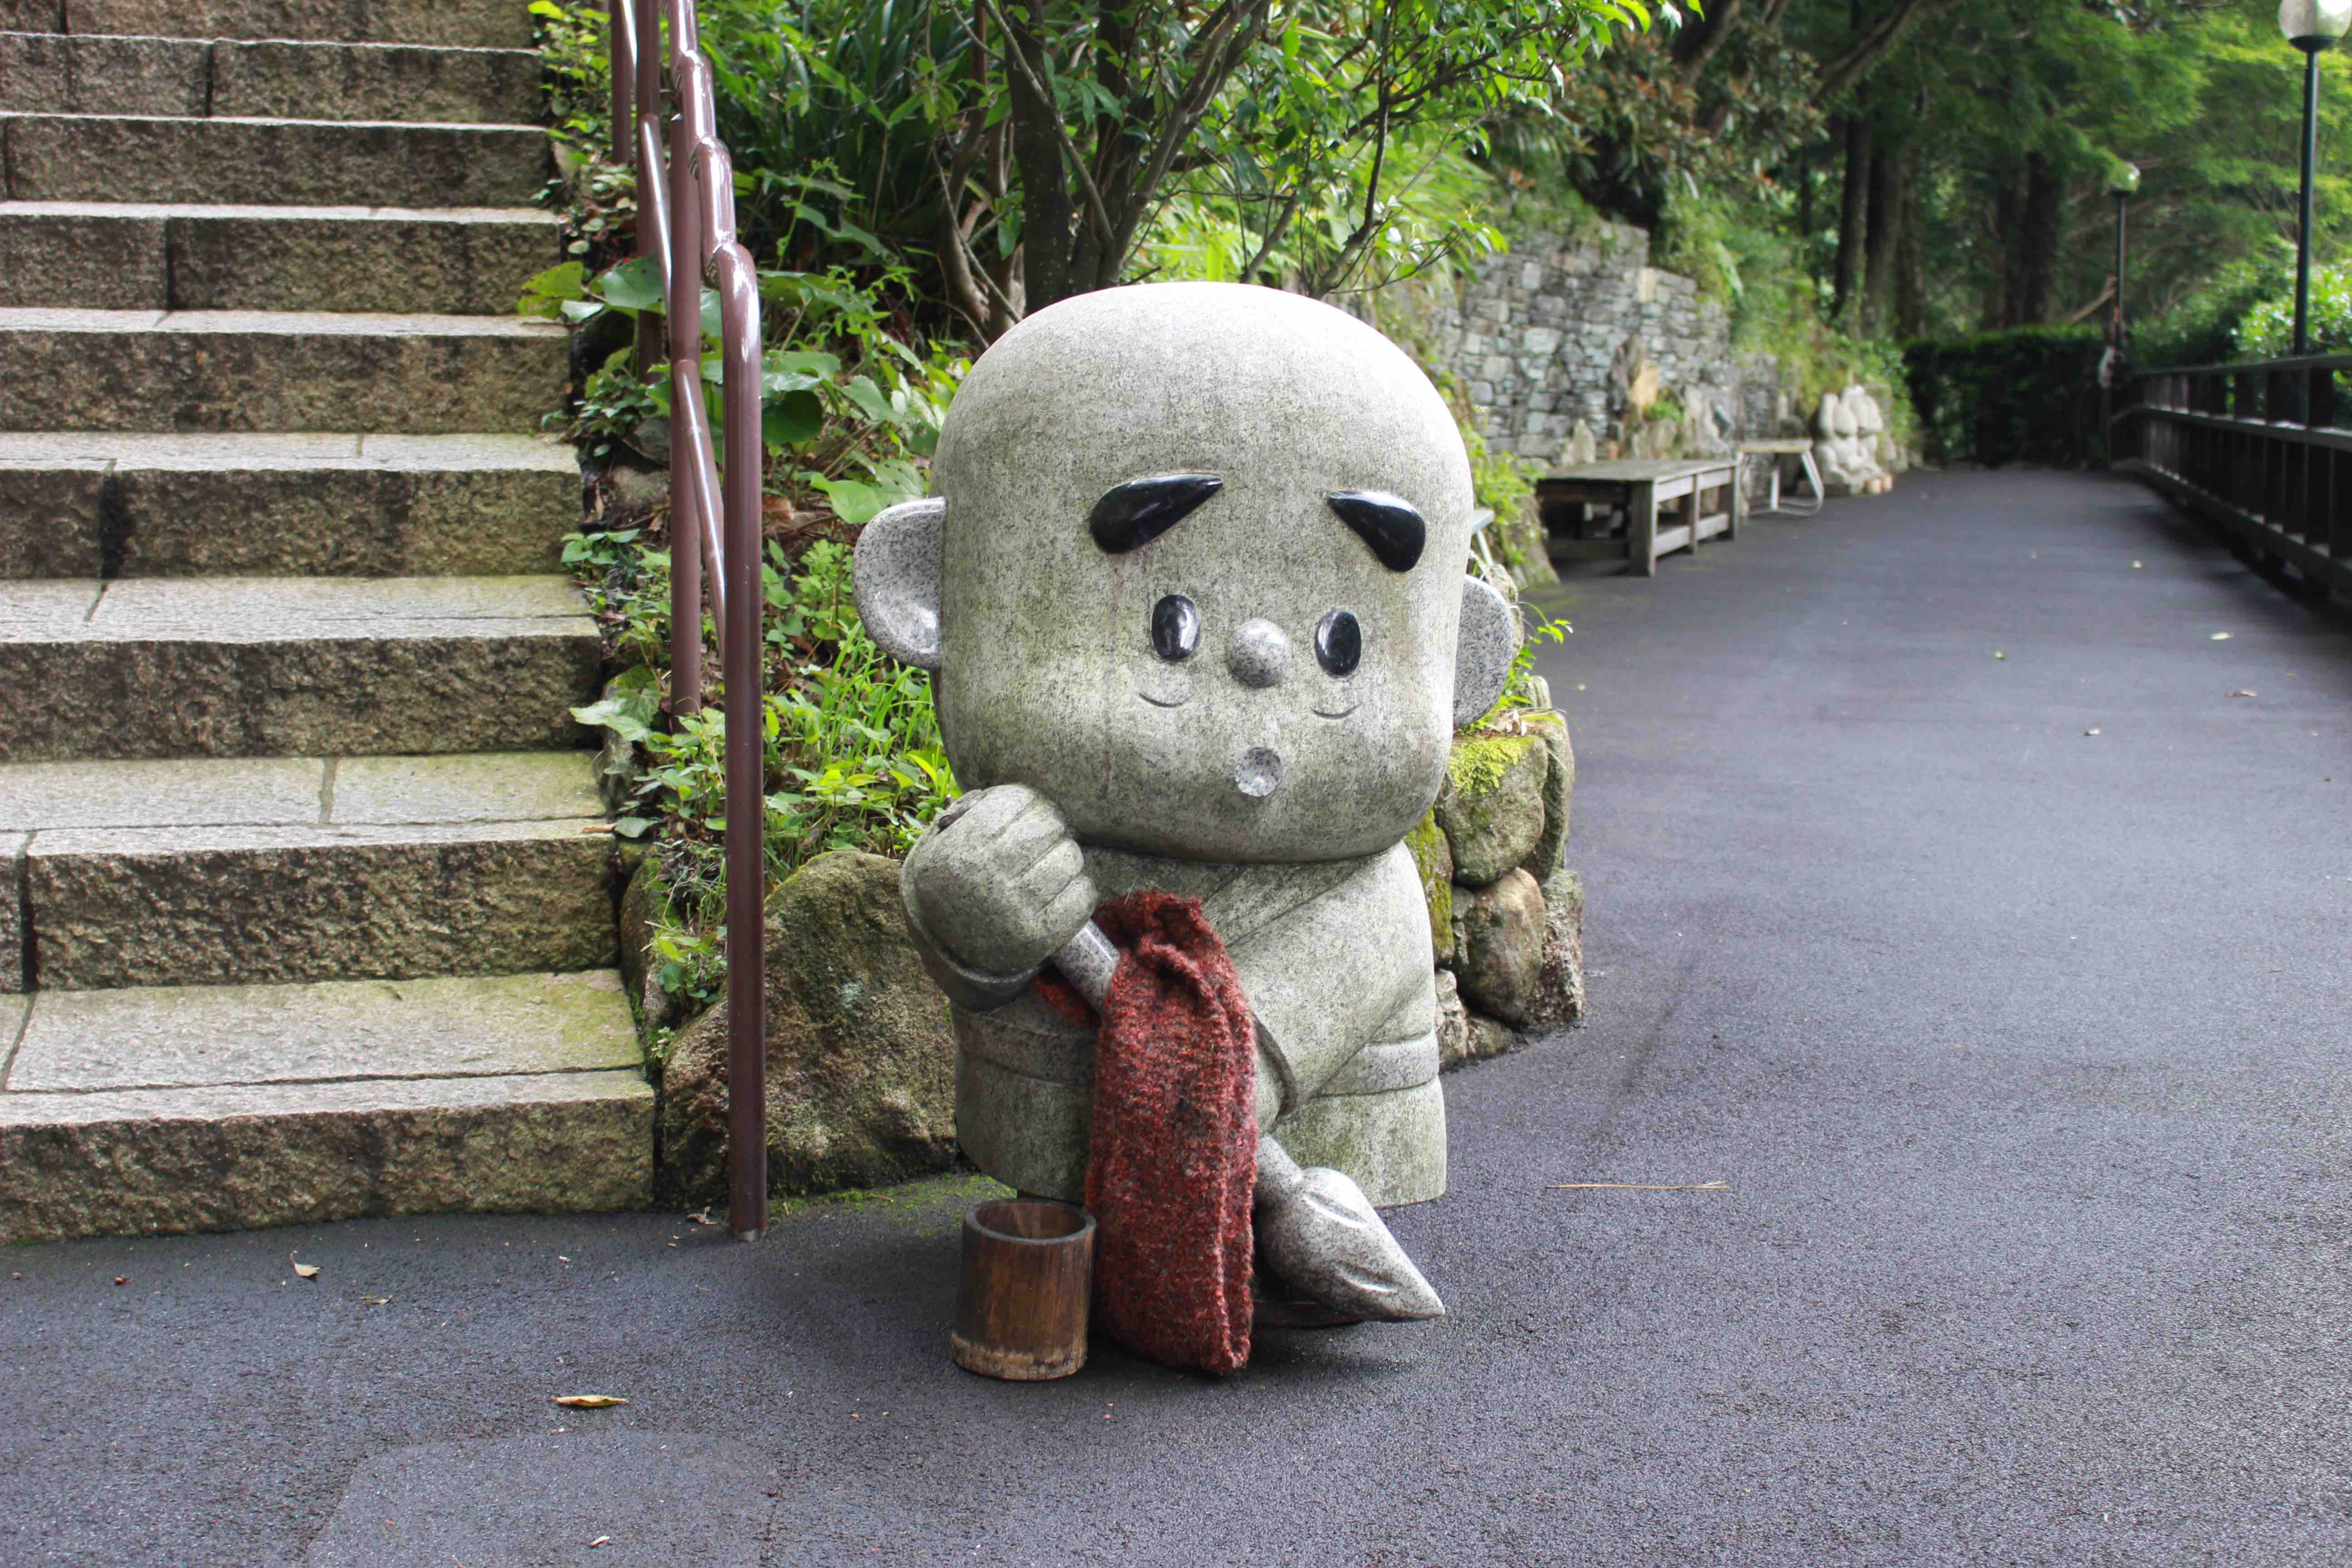
\includegraphics[scale = 0.05]{chapter2/yoshimoto.jpg}
    \caption{涅槃像見にいった時に見つけた地蔵} %タイトルをつける
    \label{fig_地蔵} %ラベルをつけ図の参照を可能にする
\end{figure}
\end{verbatim}

\begin{figure}[]
  \begin{center}
    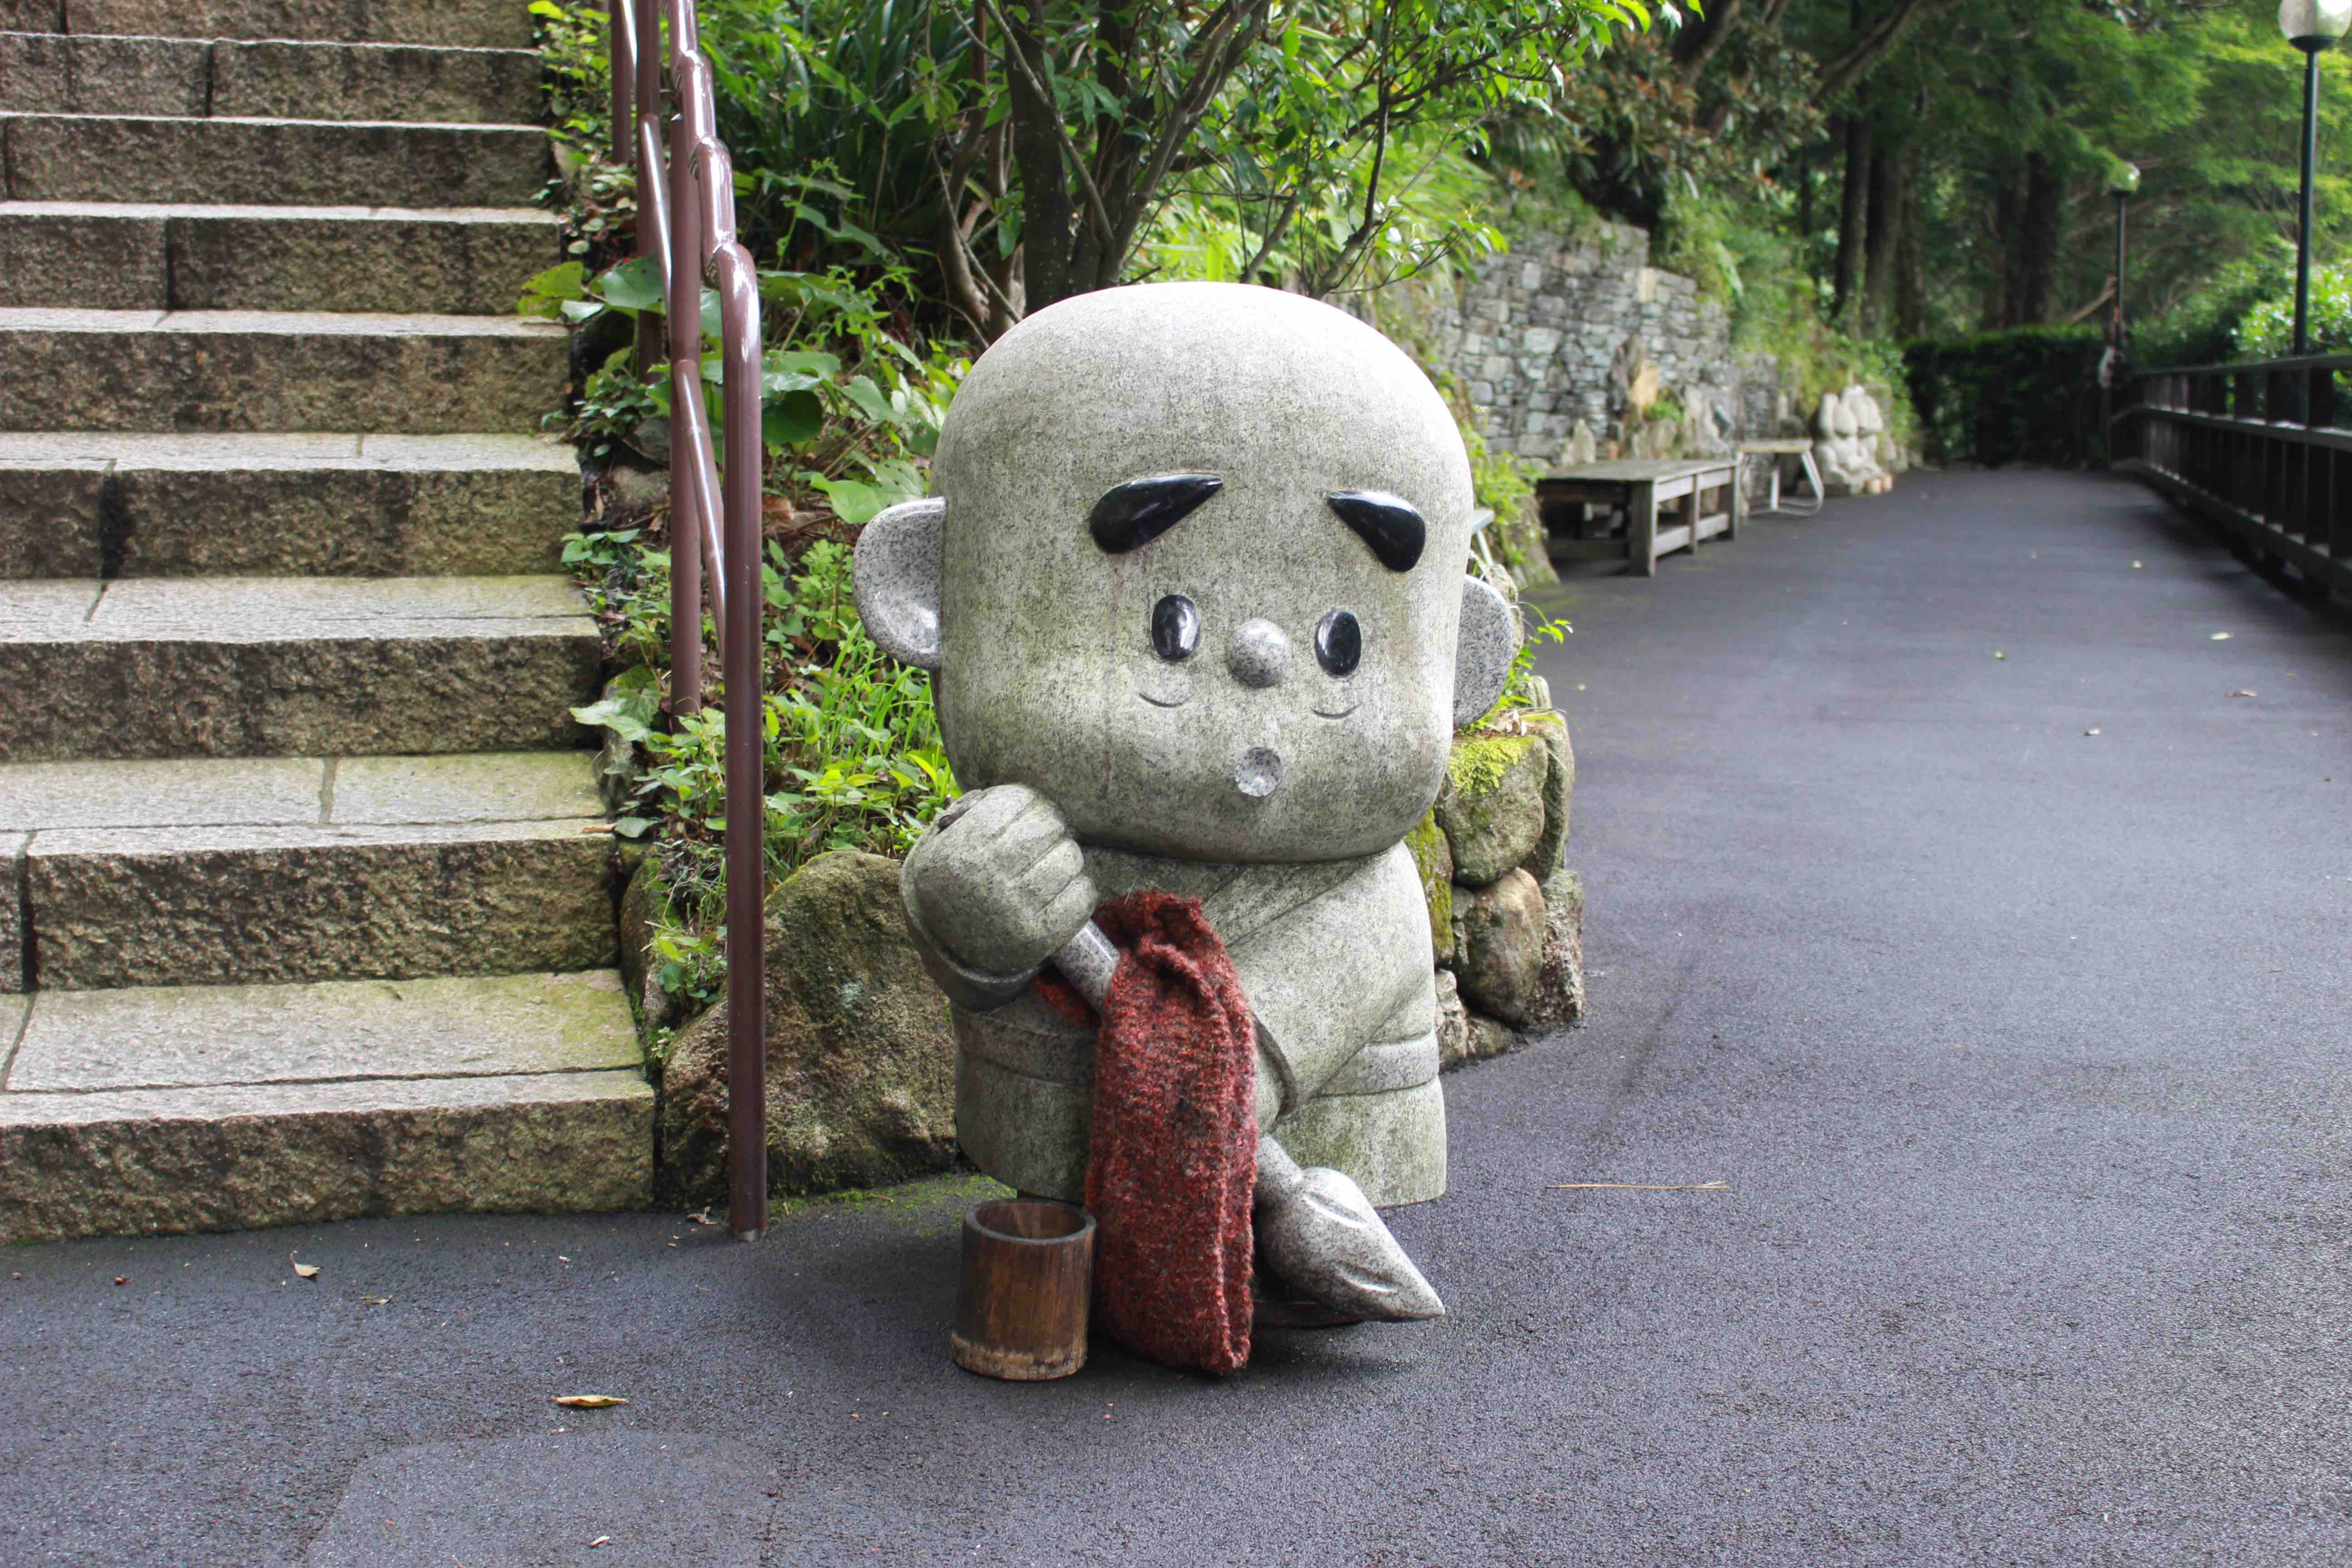
\includegraphics[scale = 0.05]{./chapter2/yoshimoto.jpg}
    \caption{涅槃像見にいった時に見つけた地蔵}
    \label{fig_地蔵}
  \end{center}
\end{figure}

\section{表}
表は結構説明が面倒なので詳細は省きます.
基本的には以下のコマンドで表が出力できます.
TeXで表を書くのは結構面倒です.
\begin{verbatim}
\begin{table}[位置指定]
  \begin{tabular}{列指定}
    表本体・・・
  \end{tabular}
\end{table}
\end{verbatim}

表本体の項目は「\verb|&|」を使って分けます.
また,数式などでも共通ですが,「\verb|\\|」を使って行を変えます.
ここでは簡単に以下の表を出力します.
\begin{verbatim}
\begin{table}[htbp]
  \centering
  \caption{Add caption}
    \begin{tabular}{l|l}
    \multicolumn{2}{c}{master unko} \\ \hline
    unko & unko2 \\
    test & test2 \\
    \end{tabular}
  \label{tab_addlabel}
\end{table}
\end{verbatim}

\begin{table}[htbp]
  \centering
  \caption{適当な表}
    \begin{tabular}{l|l}
    \multicolumn{2}{c}{master unko} \\ \hline
    unko & unko2 \\
    test & test2 \\
    \end{tabular}
  \label{tab_addlabel}
\end{table}

\section{箇条書き}

時には箇条書きをすると見やすくなることがあります.
そんな時は以下のようにするのです.

\begin{verbatim}
\begin{itemize}
    \item unko
    \item test
\end{itemize}
\end{verbatim}

出力結果は以下のようになります.
\begin{itemize}
    \item unko
    \item test
\end{itemize}

\section{参考文献}

参考文献はbibTeXを使うと大変便利です.
みんな積極的に使っていこう.
本テンプレートではref.bibという名前のファイルを作って,その中に記述してます.
詳細はWebを見ていただけたらと思います.
bibTeXはファイル内で実際に使っていない参考文献が書いてあっても,順番がめちゃくちゃであっても,TeXをコンパイルすれば順番通りかつ必要な文献だけ記載してくれます.

参考文献の実際の引用は\verb|\cite{}|を使います.{}の中にはラベルを書きます.
本テンプレートでは適当にref.bibに書き込んである参考文献のラベルを「\verb|ref_tex|」としているので,\verb|\cite{ref_tex}|と書きます.
\begin{itemize}
    \item 例)先行研究としてこんなのが提案されてる\cite{ref_tex}.
\end{itemize}
もし複数の参考文献を参照したい場合は\verb|\cite{label_1,label_2,...}|のようにラベルを「,」で区切ります.

ちなみに論文は有料でPDFがDLできないけどbibTeXならDLできたりします.
その中身をref.texにコピーして形を整えてあげると良いです.
